% !TeX program = xelatex
\documentclass[11pt,english]{article}
\usepackage[T1]{fontenc}
\usepackage{geometry}
\geometry{verbose,tmargin=2.5cm,bmargin=2.5cm,lmargin=2.5cm,rmargin=2.5cm}
\usepackage{color}
\usepackage{amsmath}
\usepackage{setspace}
\PassOptionsToPackage{normalem}{ulem}
\usepackage{ulem}
\usepackage{url}
\onehalfspacing
\usepackage{babel}
\usepackage{placeins}
\usepackage{float}
\usepackage{hyperref}

%\usepackage{mathtools}
\usepackage{fourier}            % set math font
%\usepackage{newpxmath}
\usepackage{bm} %bold math
\usepackage{fontspec}
\setmainfont{Times}
\setsansfont{Optima}
\renewcommand{\familydefault}{\sfdefault}
\usepackage{sectsty}
\allsectionsfont{\fontspec{Optima}}
\title{14.03 Recitation 5: Welfare Computations and Tax Incidence}
\author{Andrea Manera}
\date{Spring 2020}
\begin{document}
\maketitle

\section*{Outline}
In this Recitation, we will first review welfare computations. This will be a review for those of you who took 14.01, but will generally be useful to organize ideas. We will then review the application of welfare computations to the problem of tax incidence. Finally, we will discuss the economic theory foundation for using the change in consumer surplus (area under the Marshallian demand) as a welfare measure. You should see this last part as ``bonus'', and as an---hopefully interesting---application of consumer theory. Throughout the class, we will just make the appropriate assumption to use the change in consumer surplus as a welfare measure. Namely, we will always assume that \emph{income effects are small}.

\setcounter{section}{0}

\section{Welfare computations review and formulas}

\subsection{Preamble: what is an opportunity cost?}

To understand welfare computations, we must first face the question of defining what opportunity-cost is. Succinctly, this is the alternative use of the resources that each part brings to the market in an exchange. In particular, when thinking of a market for a specific good, the consumer can use each of her dollars to buy some other bundle of goods rather than the good in question. On the other hand, the producer might use her resources, for example labor, to produce some other good or enjoy leisure time. Thus, both parts will benefit from the exchange as long as the value they obtain from each unit involved in such exchange is higher than their opportunity-cost. For the consumer, this means that each unit purchased should deliver a utility (measured in dollar terms) that is higher than what she would get buying other goods for the same amount. This is encoded in the demand curve. We have seen in class that, by Shephard lemma, the area under the Hicksian demand is the consumer's valuation of the units purchased.\footnote{Recall that Shephard's lemma states that the integral of the Hicksian demand is the expenditure function. Therefore the area under the Hicksian demand is how much the consumer would like to spend for the unit purchased to achieve a certain level of utility.}. For the producer, this means that, for each of the units supplied, she needs to receive a compensation at least equal to her outside option. This outside option is encoded by the supply curve.\footnote{We can think that the producer is just another consumer who is sacrificing resources to produce the good. In keeping with the above reasoning, she will only want to produce for the exchange if she obtains from it at least the resources she uses in production.} 

A less succinct, but extremely fascinating, explanation of the term is given in the following quote, from the article where the term opportunity-cost was coined:\footnote{Green, David I. 1894. Pain-Cost and Opportunity-Cost. \textit{The Quarterly Journal of Economics}.  }

\begin{quote}
``That the exchange value of commodities which are subject
to free competition tends to correspond with the cost of production
has been recognized from the beginning of economic
theory, and must in some sense be true. But what is commonly
summed up in the term " cost" is not principally the pain
of weariness on the part of the laborer, and of long delay in
consumption on the part of the capitalist; but the cost consists
for the most part of the sacrifice of opportunity. A certain
man cannot afford to keep books at \$100 a month. Why?
Because he can earn \$200 as superintendent of the shops. Another
or the same man cannot afford to work over six days in
the week, because such action would deprive him of important
opportunities for pleasure and advancement. A fanner cannot
afford to use a certain lot for pasture, because it yields him
greater profit as meadow. The laborer stops work at a certain
hour, not simply because he is tired, but because he wants
some opportunity for pleasure and recreation. That which
gives a man strength in his demand for higher pay is the fact
that he is able to secure higher pay elsewhere. By devoting
our efforts to any one task, we necessarily give up the opportunity
of doing certain other things which would yield us some
return; and it is, in general, for this sacrifice of opportunity
that we insist upon being paid rather than for any pain which
may be involved in the work performed.''
\end{quote}

The article was in the context of the debate of whether marginal utility or marginal cost determined the exchange value of things, and the author was arguing against simplistic theories of what this marginal cost is in the context of labor markets. His main target is another economist who came up with the term ``pain-cost'', which I wonder why ended up having a lot less success\dots\footnote{It was also a rather nonsensical theory. The theory opposed to Green's argued that the opportunity-cost of labor was effectively the pain put in producing the thing, thus neglecting the outside option of not producing the object of the exchange. Since I enjoy teaching, I would probably get no money according to it, although I did get a few unpleasant paper cuts scanning midterms.}

\subsection{Computing Welfare}

How do markets generate welfare? Because the two parts involved in exchange obtained a benefit that is above the opportunity-cost of resources used in the exchange.

For consumers, the benefit is the marginal utility from the good considered, measured in dollars, of each unit purchased. The opportunity-cost is the expenditure on the good purchased, which cannot be allocated to other goods who give at least that utility in dollar terms (if you spent \$10 on apples, you cannot spend those \$10 on bananas). For producers, the benefit is the revenue from each unit (the market price). The opportunity-cost is the alternative use of resources needed to produce the good. An apple farm could use the land for some other use, and her time to enjoy leisure other than farm, or look for another job, etc.

How do we get these measure from a supply and demand graph? 


Let us start with the demand curve $D(p)$. This curve expresses the valuation of consumers for each additional unit locally. Technically, this would have to be a Hicksian demand, as you will see below. Hicksian demands are hard to measure, though, so we often use the Marshallian demand and assume income effects on that good are small.

 You can think of the demand curve being downward-sloping in two ways:
\begin{enumerate}
	\item The economy is made up by many agents who have different valuations for the good. On the graph, you sort these consumers by their valuation. The first unit is the one consumed by the agent with the highest valuation, the second unit by the consumer with the second-highest valuation and so on. The last agent to buy goods on the market is the one for which the valuation of the good exactly equals the market price.
	\item The economy is ``one big family'' made up of all agents. The more units of some good you give the family, the less their utility/valuation from marginal increases in the good, as a result of decreasing MRS.\footnote{Remember the Hicksian demands for consumers in the food stamp case: the more food I give you, the less you value it relative to other goods.}
\end{enumerate}
In both cases, each of the exchanges carried out creates a sort of ``utility surplus'' for all consumers/units except the last one. Indeed, the demand curve, which represent consumers' valuation, is above the equilibrium price up to the equilibrium quantity, so the consumers value each of the units before the very last they purchase above the market price. Thus, the presence of the market allows them to ``transform'' their dollars (which are worth exactly the market price in terms of other goods) into utility, obtaining a ``utility profit'' on each unit purchased. This profit equals the difference between their own valuation, the demand curve, and the market price. From this discussion, we can define a measure of the welfare of consumers generated by exchanges as the area that lies between the equilibrium price and consumers' demand. We can see this in Figure \ref{fig:CS}.

In Figure \ref{fig:PS} we see an analogous reasoning for the producer. The opportunity-cost is now given by the area \emph{below} the supply curve, which measures how resource could have been used. If this good were produced with labor, we could think of the leisure time given up among other things.

Figure \ref{fig:SS} puts it all together and gives the expressions that correspond to these surpluses. Consumer surplus is given by the integral of the inverse demand curve, $D(p)$, between the market price and infinity, while producer surplus is given by the integral of the inverse supply curve, $S(p)$, from the minimum price at which some good is supplied up to the market price, $p_{mkt}$.

\begin{figure}[htpb!]
	\centering
	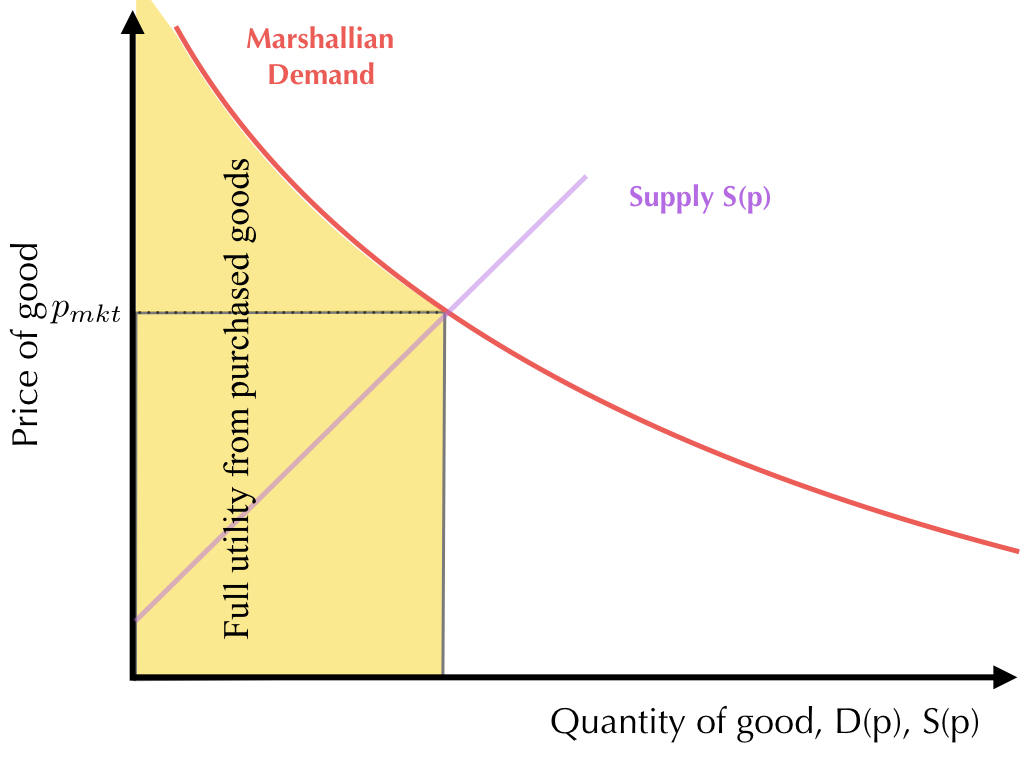
\includegraphics[width=0.5\linewidth]{Figures/CS1}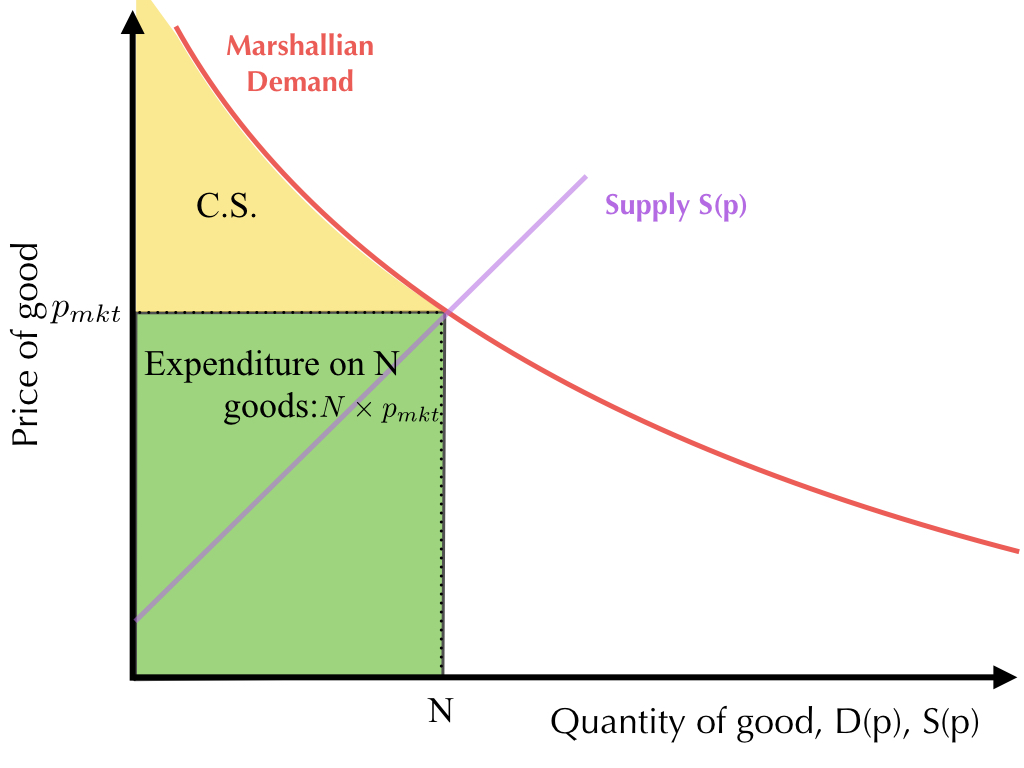
\includegraphics[width=0.5\linewidth]{Figures/CS2}
	\caption{Consumer Surplus}
	\label{fig:CS}
\end{figure}

\begin{figure}[htpb!]
	\centering
	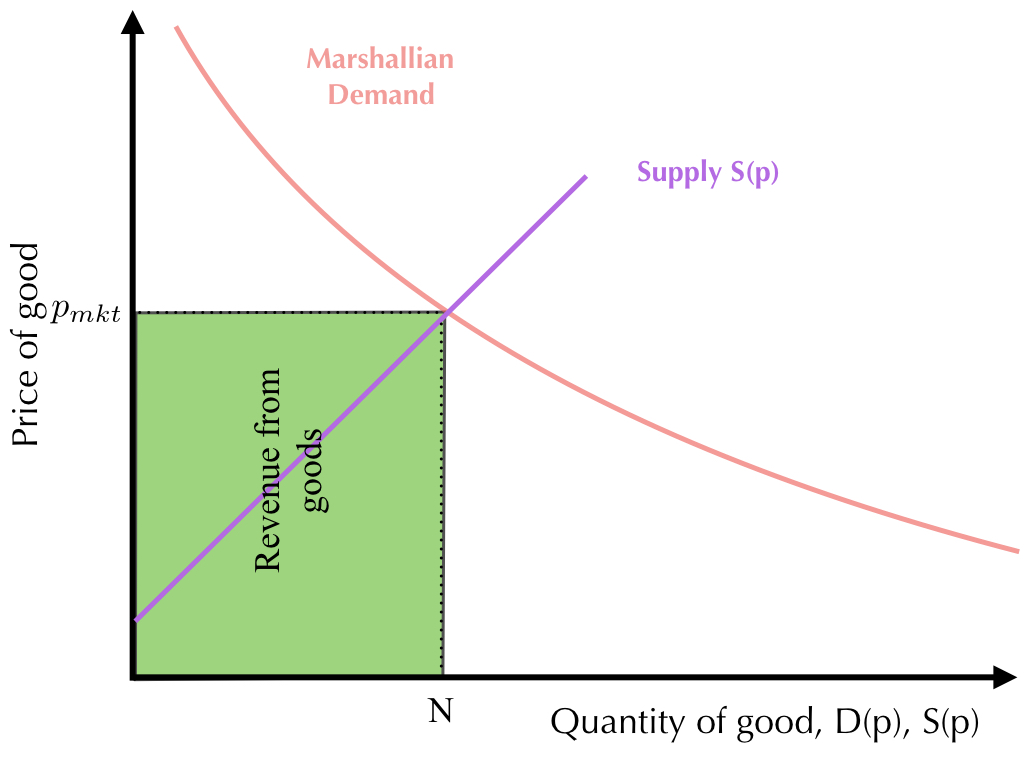
\includegraphics[width=0.5\linewidth]{Figures/PS1}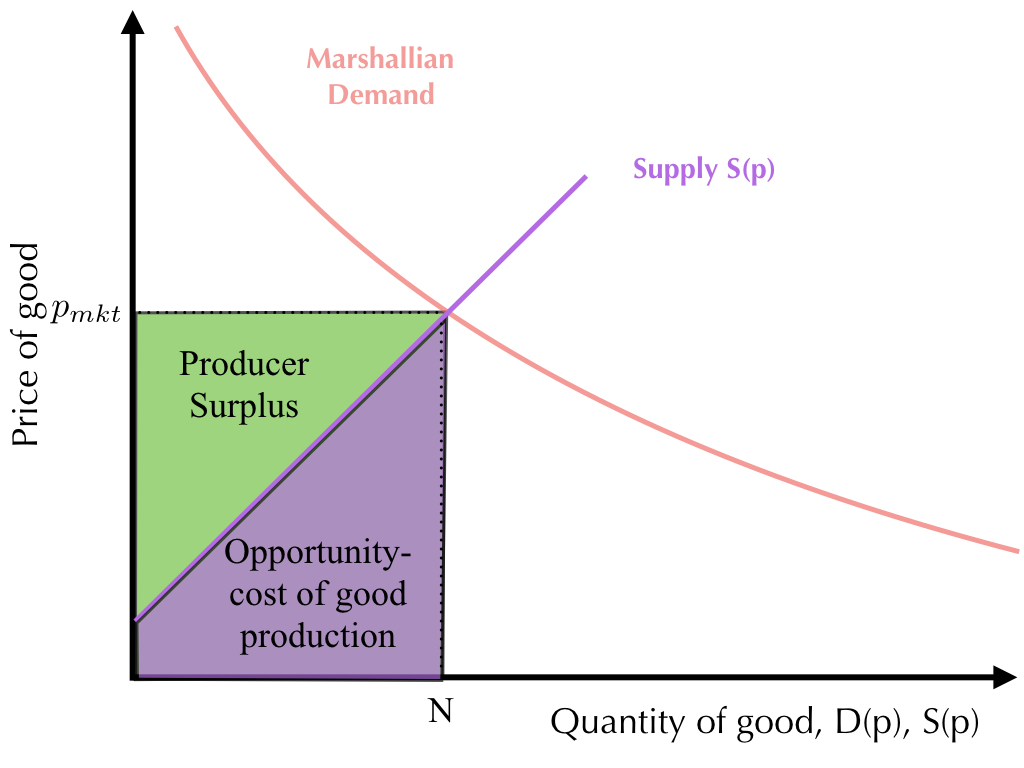
\includegraphics[width=0.5\linewidth]{Figures/PS2}
	\caption{Producer Surplus}
	\label{fig:PS}
\end{figure}

\begin{figure}[htpb!]
	\centering
	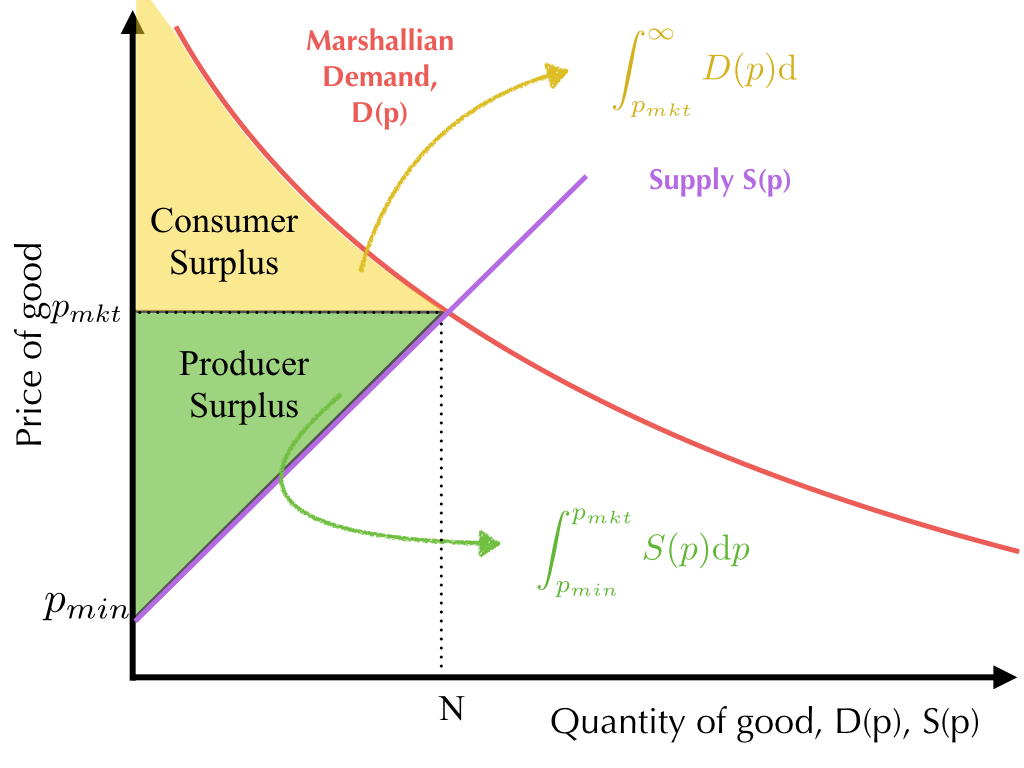
\includegraphics[width=0.8\linewidth]{Figures/SS}
	\caption{Surplus expressions}
	\label{fig:SS}
\end{figure}


\FloatBarrier
\subsection{Tax incidence}

Let us now move to the effect of taxes on welfare. As we saw above, the market generates a surplus for consumers and producers \emph{as a result of the exchanges that are carried out}. Taxes act on this welfare in two ways:
\begin{enumerate}
	\item They redistribute the welfare between three main agents: agents who demand the good, agents who supply the good, and the government;
	\item They \emph{can} reduce the overall surplus generated by exchanges, causing a \emph{deadweight loss}. 
\end{enumerate}
When looking at welfare, we have to keep in mind both aspects. Below we will see a case where there is both a redistribution and a deadweight loss created by a tax. But there are other cases where tax-like policies only generate a redistribution, and no welfare loss. This is the case when other deviations from competitive markets are already present. We have seen this with monopsony in labor markets. Starting from a situation without the minimum wage, we can increase welfare by introducing one, because this increases the quantity of exchanges in the market (in this case the quantity is given by employment). A welfare gain will come as long as the new minimum wage increases employment, \textit{regardless of whether this new wage is above the market-clearing level}. Of course, the welfare gains will accrue to workers, while the monopsonist will suffer a reduction in profits.\footnote{It is important here to remember that we use a so-called ``utilitarian'' welfare measure, where we sum the surplus of all agents in the economy to obtain social welfare. However, there are other measures that would have different implications. For example \textit{min-max} welfare measures take the minimum of the surplus of each agent, favoring more egalitarian allocations. Do check out Wikipedia on this topic if you are curious: \url{https://en.wikipedia.org/wiki/Social_welfare_function}.} 

When we start from a competitive market, however, the analysis is much simpler. A tax acts like a \textit{wedge} that prevents demand and supply curves from meeting at the competitive market level (thinks of the two curves like two doors which open in opposite directions). This will cause a social welfare loss given by the reduction in exchanges carried out. How many exchanges are lost will depend on how price-elastic are the two sides of the market. If they are very price-elastic (which translates in flatter curves on the space where $p$ is on the y-axis and quantity on the x-axis), they will reduce more the quantity demanded and supplied for any given wedge introduced between them. The more elastic are the curve, the more exchanges will be lost. Geometrically, this makes sense, as the height of the wedge is given by the tax, and if the two curves are very flat, we will have to move back along the x-axis a lot to obtain a vertical distance large enough to insert the tax wedge in between the two curves.

Moving to distribution, the tax will affect more the side of the market that is less price elastic, while the price-elastic side will adjust more on quantities and pay less of the overall tax burden at the new equilibrium price and quantity. To fix ideas, think of a very necessary good, like a life-saving medicine. In this case, consumer will likely be available to pay any price to get the quantity they need. Therefore, if you tax this medicine, the quantity demanded by consumers will not change at all, and they will pay the additional tax without moving the along the supply curve. Producers will not feel the tax at all, as they will suffer no quantity reduction even charging the exact same pre-tax price as the one they were charging above. The final agent we have to account for is the government. If we think that this is benevolent and will give back the resources raised to consumers and producers (for example in the form of public goods), we have to count tax revenue among the components of social welfare. Figure \ref{fig:tax1} shows how inserting the wedge affects consumer and producer surplus.

\begin{figure}[t!]
	\centering
	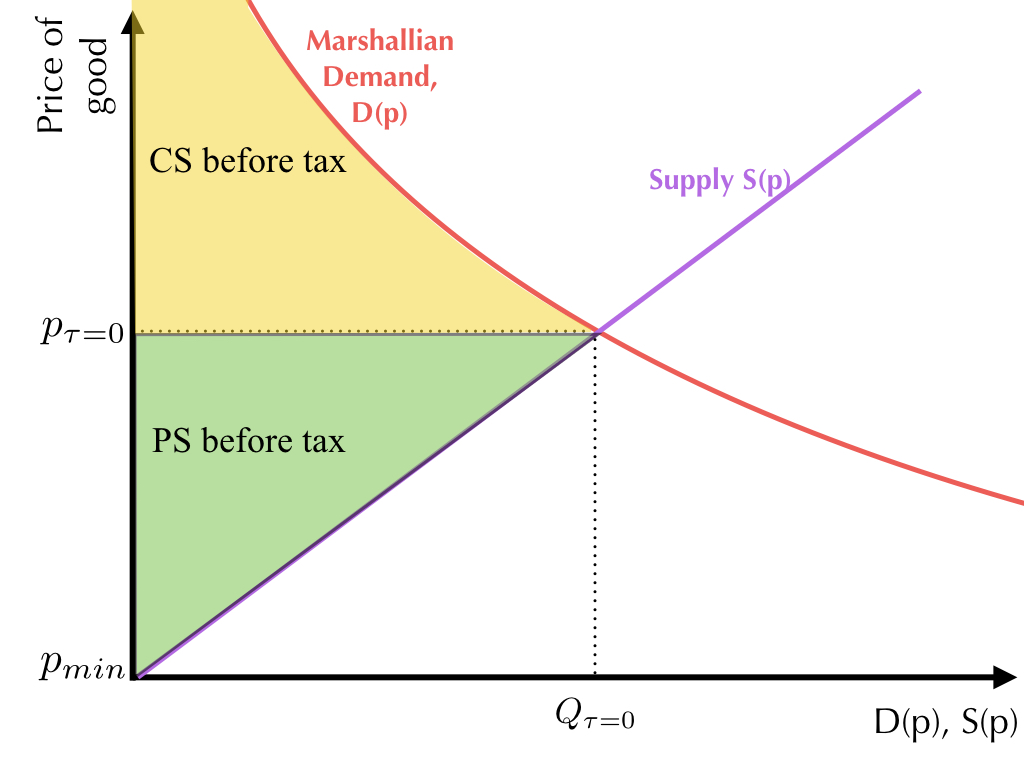
\includegraphics[width=0.5\linewidth]{Figures/Tax1}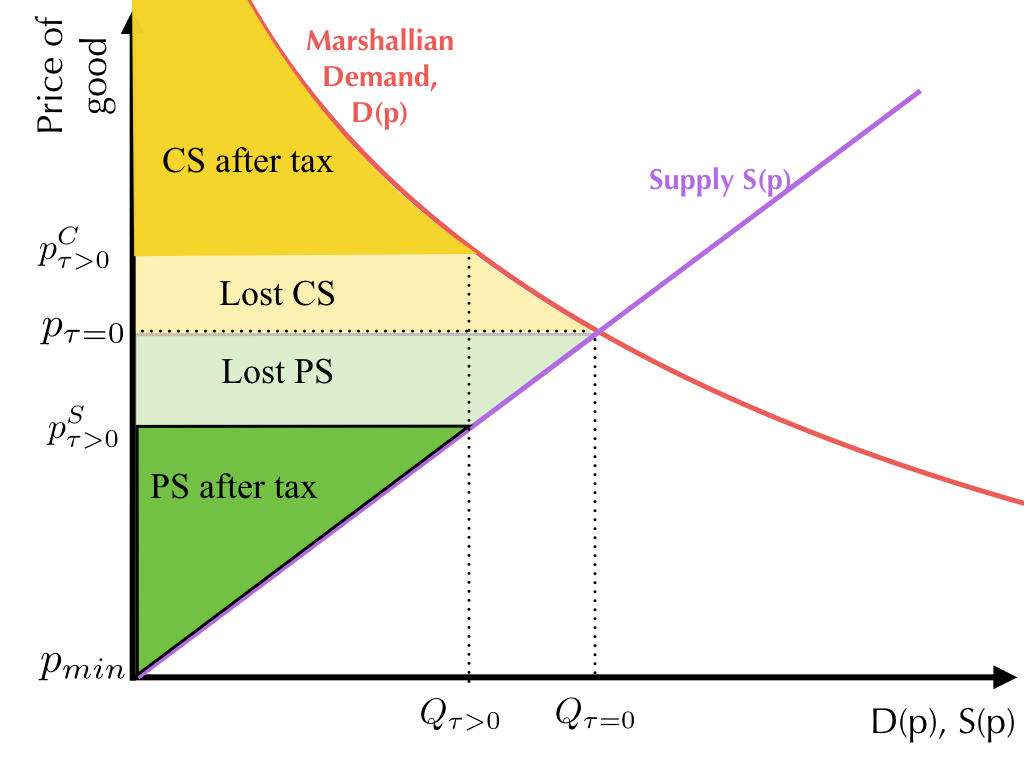
\includegraphics[width=0.5\linewidth]{Figures/Tax2}
	\caption{Inserting a tax wedge $\tau>0$ in the competitive market, starting from no-tax situation $\tau=0$. The prices $p^C_{\tau>0},p^S_{\tau>0}$ represent the prices charged to consumers and received by suppliers after the introduction of the tax, and $Q_{\tau>0}$ is the post-tax equilibrium quantity.}
	\label{fig:tax1}
\end{figure}




Then what is the deadweight loss? Once again, this is all the trades we lost by introducing the tax. Figure \ref{fig:wrapup} shows the split of the welfare and the DWL. We owe this analysis to economist Arnold Carl Harberger (b. 1924), so the DWL loss triangle is also called \emph{Haberger's triangle}.\footnote{His advisors were Kenneth Arrow, and Franco Modigliani, who both went on to win Nobel prizes.} 

\begin{figure}
	\centering
	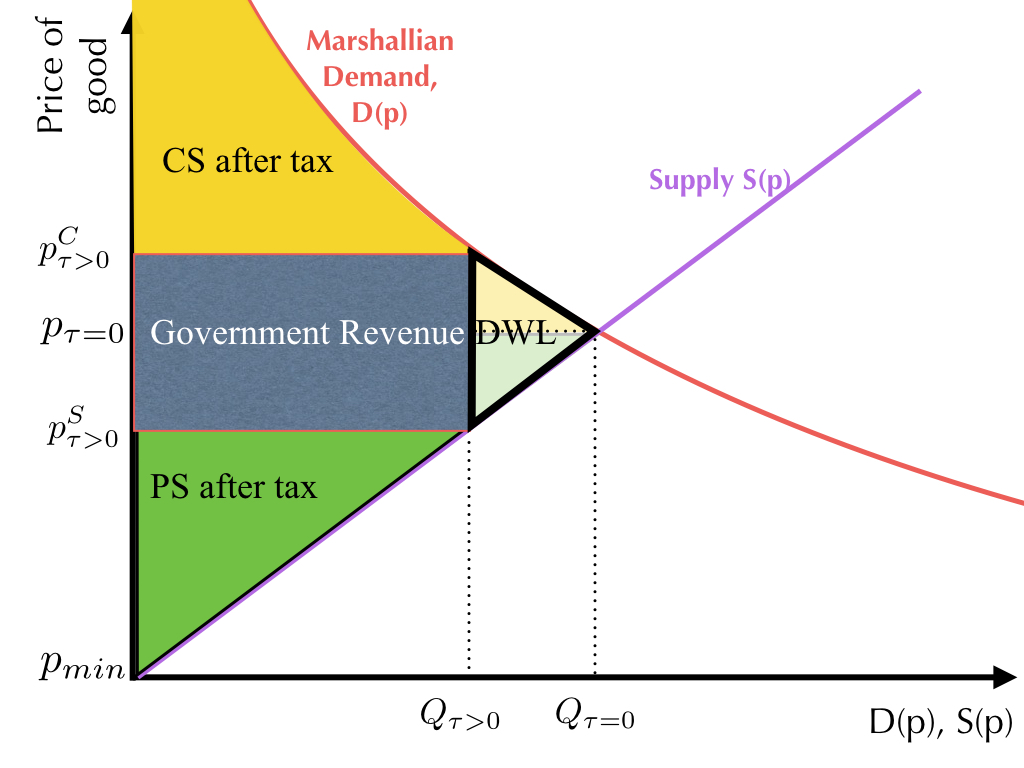
\includegraphics[width=0.5\linewidth]{Figures/Tax3}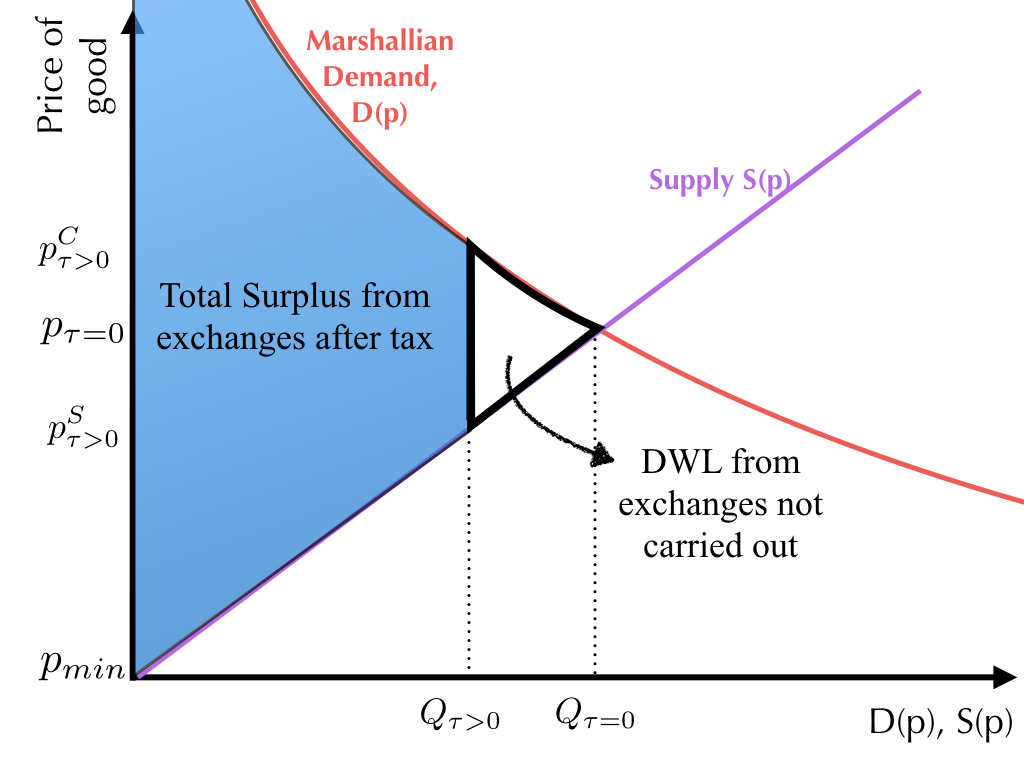
\includegraphics[width=0.5\linewidth]{Figures/Tax4}
	\caption{Welfare effects of a tax and the deadweight loss from lost exchanges.}
	\label{fig:wrapup}
\end{figure}


\section{The foundations of welfare measures}

Above we used the Marshallian demand to measure consumer welfare. In what follow, we will see why, and under what conditions, this is a good measure of welfare. This is more like a bonus part, but it is a fun application of consumer theory if you like the math behind it.

\subsection{Measuring utility in dollars}

Consider a setting with two goods $x,y$. If the price of good $x$
goes from $p_{x}$ to $p_{x}'$, how does that affect the consumers'
welfare? The answer is given by the difference between post-change
utility $U'$ and pre-change utility $U$.

If we have the indirect utility of the consumer $V(p_{x},p_{y},I)$,
the answer is $V(p_{x}',p_{y},I)-V(p_{x},p_{y},I)$. This will tell
us something like: ``utility falls by 100 utils''. However, utility
is an ordinal and subjective measure of welfare. In particular, we
can take any monotone transformation of the utility function to represent
the same preferences. This will give different indirect utilities,
which will in turn result in different answers to our original questions.
This creates problems for measuring individual welfare changes, and
even more collective welfare. In particular, since total welfare is
the sum of individual surpluses, we will have the same measurement
problem as above. In addition, we would need to choose how to weigh
individual utilities when summing them up... a real mess! 

Consumer theory provides a wonderful way to get around this issue,
since we can use the expenditure function as an indirect utility.
The advantage is that now indirect utility will now be expressed in
dollars, addressing the measurement problem above. In particular,
we can choose a vector of prices $\left(\bar{p_{x}},\bar{p_{y}}\right)$,
and define indirect utility as:
\[
E\left(\bar{p_{x}},\bar{p_{y}},V(p_{x},p_{y},I)\right)
\]
Why is this an indirect utility function?
\begin{itemize}
\item Indirect utilities have to be increasing in $I$ and decreasing in
prices;
\item Note that $E\left(\bar{p_{x}},\bar{p_{y}},U\right)$ is increasing
in $U$;
\item Therefore $E\left(\bar{p_{x}},\bar{p_{y}},V(p_{x},p_{y},I)\right)$
is just a monotone transformation of the original indirect utility,
so it is itself an indirect utility.
\end{itemize}
We refer to $E\left(\bar{p_{x}},\bar{p_{y}},V(p_{x},p_{y},I)\right)$
as a \emph{money-metric indirect utility function }(since it measures
utility in dollar terms).

Now that we have an indirect utility in dollars, we can answer our
original question by computing the welfare change in dollar terms:
\[
E\left(\bar{p_{x}},\bar{p_{y}},V(p_{x}',p_{y},I)\right)-E\left(\bar{p_{x}},\bar{p_{y}},V(p_{x},p_{y},I)\right)
\]
\[
E\left(\bar{p_{x}},\bar{p_{y}},U'\right)-E\left(\bar{p_{x}},\bar{p_{y}},U\right)
\]
Last issue: why does this solve our problems regarding the choice
of the utility function, since utility levels $U',U$ appear in the
computations? Because it is true that we can choose different utility
functions (monotone transformations) to represent the same preferences,
leading to different values of $U'$,$U$ depending on the representation
we choose. However, in order to represent the same preferences, a monotone
transformation should lead to the same bundle of goods (marshallian
demands) consumed for each price and income. This means that the expenditure
function will be the same, since, e.g.:
\[
E\left(\bar{p_{x}},\bar{p_{y}},U'\right)=E\left(\bar{p_{x}},\bar{p_{y}},V(p_{x}',p_{y},I)\right)=\bar{p_{x}}d_{x}(p_{x}',p_{y},I)+\bar{p_{y}}d_{y}(p_{x},p_{y},I)
\]
where $d_{x}$,$d_{y}$ are Marshallian demands. Since Marshallian
demands for monotone transformations of a utility function are the
same, it follows that the choice of the underlying utility will not
matter for the computation of the money-metric utility function. (You
can convince yourself by computing Marshallian demands for $U(x,y)=x^{\alpha}y^{1-\alpha}$,
and its monotone transformation $\hat{U}(x,y)=x^{2\alpha}y^{2(1-\alpha)}$).

\subsection{Three welfare measures}

The above discussion provided us with a utility-free measure of welfare.
There is only one last choice to make, in order to compute the measure
of welfare using money-metric utility: the vector $\left(\bar{p_{x}},\bar{p_{y}}\right)$.
The obvious candidates are:
\begin{itemize}
\item Prices after the change: $\left(p_{x}',p_{y}\right)$. The change
in welfare is:
\[
E\left(p_{x}',p_{y},U'\right)-E\left(p_{x}',p_{y},U\right)=E\left(p_{x}',p_{y},V(p_{x}',p_{y},I)\right)-E\left(p_{x}',p_{y},V(p_{x},p_{y},I)\right)=I-E\left(p_{x}',p_{y},V(p_{x},p_{y},I)\right)
\]
Where the last equality comes from duality properties.\footnote{By non-satiation, the minimum I can spend to get the maximum utility
at $p_{x},p_{y}$ with income $I$, $V(p_{x},p_{y},I)$ is \emph{all
my income} $I$} They also imply that:
\[
I=E\left(p_{x},p_{y},V(p_{x},p_{y},I)\right)=E\left(p_{x},p_{y},U\right)
\]
Finally, we can use this to express the change in welfare as:
\[
E\left(p_{x},p_{y},U\right)-E\left(p_{x}',p_{y},U\right)
\]
This is known as \textbf{Compensating Variation. } It answers the question:
how much money does the consumer need to \emph{lose }after the price
change in order to get the same utility as before? How much income
do I have to \emph{take} from the consumer in order to \emph{compensate}
them for the price increase? So the consumer is as happy as before
the price change if they receive \textbf{minus} the compensating variation
\textbf{together with the price change}. 
\item Prices before the change: $\left(p_{x},p_{y}\right)$. The change
in welfare is:
\[
E\left(p_{x},p_{y},U'\right)-E\left(p_{x},p_{y},U\right)=E\left(p_{x},p_{y},V(p_{x}',p_{y},I)\right)-E\left(p_{x},p_{y},V(p_{x},p_{y},I)\right)=E\left(p_{x},p_{y},V(p_{x}',p_{y},I)\right)-I
\]
Where the last equality comes from duality properties. They also imply
that:
\[
I=E\left(p_{x}',p_{y},V(p_{x}',p_{y},I)\right)=E\left(p_{x}',p_{y},U'\right)
\]
(By non-satiation, the minimum I can spend to get the maximum utility
at $p_{x}',p_{y}$ with income $I$ is \emph{all my income} $I$).
Finally, we can use this to express the change in welfare as:
\[
E\left(p_{x},p_{y},U'\right)-E\left(p_{x}',p_{y},U'\right)
\]
This is known as \textbf{Equivalent Variation. } It answers the question:
how much money is the consumer willing to \emph{lose} in order to
avoid the price change? How much money do I need to \emph{give }the
consumer in order to make cause a utility change that is \emph{equivalent}
to the price change? So the consumer is as happy as after the price
change if they \textbf{get} the compensating variation and \textbf{no
price change occurs}. 
\end{itemize}
Two important points:
\begin{enumerate}
\item Which measure shall we use? It depends on what we are looking at.
For example, CV is useful to know how much we should transfer to affected
consumers if we planned a change (e.g. we decided to build a highway,
how much money do we have to give to people who live close to it to
compensate them for the noise/pollution). EV is instead useful for
cost-benefit analysis, in particular if we are considering whether
to implement a change that benefits a part over another. In the example
above, suppose that the benefits of the highway are lower than the
EV. EV is a measure of the costs so maybe I do not want to build it. I particular I could tax consumers for the amount of benefits of the highway (less than EV) and transfer the proceeds to whoever would have benefited from it. This would leave everyone better off than under the original highway-building scenario.
\item Computation: use Shephard's lemma for a graphical representation.
In particular, we can express
\[
E\left(p_{x},p_{y},U'\right)=\int_{p_{x}}^{\infty}\frac{\partial E\left(p,p_{y},U'\right)}{\partial p_{x}}dp=\int_{p_{x}}^{\infty}h_{x}(p,p_{y},U')dp
\]
which also implies
\[
EV=E\left(p_{x},p_{y},U'\right)-E\left(p_{x}',p_{y},U'\right)=\int_{p_{x}}^{\infty}h_{x}(p,p_{y},U')dp-\int_{p_{x}'}^{\infty}h_{x}(p,p_{y},U')dp=\int_{p_{x}'}^{p_{x}}h_{x}(p,p_{y},U')dp
\]
Analogously:
\[
CV=\int_{p_{x}'}^{p_{x}}h_{x}(p,p_{y},U)dp
\]
i.e. areas to the left of the Hicksian demand curve corresponding
to the final and initial utility level respectively. 
\end{enumerate}
Summing up, the money-metric measures of welfare changes are:
\begin{itemize}
\item \textbf{Compensating variation: }How much I should take from the consumer
to make her as happy as before the price change at new prices? 
\[
CV=\int_{p_{x}'}^{p_{x}}h_{x}(p,p_{y},U)dp
\]
\item \textbf{Equivalent: }How much I should take from the consumer to make
her as happy as after the price change at old prices? 
\[
EV=\int_{p_{x}'}^{p_{x}}h_{x}(p,p_{y},U')dp
\]
\end{itemize}
To these two, we can add a third welfare measure, built by analogy
to the above two - and more useful since it is hard to estimate the
Hicksian demand -: the \textbf{Change in Consumer Surplus ($\Delta$CS),
or Area Variation (AV):}
\begin{itemize}
\item It is given by the area to the left of the Marshallian demand:
\[
\Delta CS=\int_{p_{x}'}^{p_{x}}d_{x}(p,p_{y},I)dp
\]
and answers the question: what is the difference between the willingness
to pay (WTP) and the price for the units that would have been traded
if it were not for the price increase?
\end{itemize}
When is such measure a good utility measure, i.e. when is it close
to money-metric utility? When income effects are small, in which case
Hicksian and Marshallian demand are close (think of the income effect
in the Slutsky equation). This is more likely to hold if the quantity
of the good consumed is not too high to start with, so that the price
increase does not affect \emph{real} income too much.

In general, we have the following relations. For a price increase/decrease:
\begin{itemize}
\item $\mid CV\mid\geq\mid\Delta CS\mid\geq\mid EV\mid$ for a normal good;
\item $\mid CV\mid\leq\mid\Delta CS\mid\leq\mid EV\mid$ for an inferior
good.
\end{itemize}
The absolute values are there because, for a price decrease, all this terms have positive signs (think about the fact that decreasing a price must increase consumers' welfare), while for a price increase they all have a negative sign, so the chain of inequalities will revert.

\subsection{Graphical representation}

We will now convince ourselves that the above inequalities are correct
and visualize these areas. Preliminarily, remember that:
\begin{itemize}
\item Hicksian demand is steeper than Marshallian for a normal good;
\item Hicksian demand is flatter than Marshallian for an inferior good.
\end{itemize}
This comes from the Slutsky equation:

\[
\frac{\partial h_{x}}{\partial p_{x}}=\frac{\partial d_{x}}{\partial p_{x}}+\frac{\partial d_{x}}{\partial I}h_{x}
\]
Thus:
\[
\frac{\partial h_{x}}{\partial p_{x}}\geq\frac{\partial d_{x}}{\partial p_{x}}\qquad\text{iff}\qquad\frac{\partial d_{x}}{\partial I}h_{x}\geq0
\]
(positive income effect, i.e. normal good). If you increase the price
of a good you will have a larger decrease in the Marshallian demand.
This is because not only you want to substitute away from the good,
but you also want less because your real income is lower.

Also remember that Hicksian and Marshallian demand coincide in particular
instances. In particular, for given prices $\left(\bar{p_{x}},\bar{p_{y}}\right)$,
and income $I_{0}$, define $U_{0}\equiv V(\bar{p_{x}},\bar{p_{y}},I_{0})$,
then $d_{x}(\bar{p_{x}},\bar{p_{y}},I_{0})=h_{x}(\bar{p_{x}},\bar{p_{y}},U_{0})$.
This is very useful to draw our figures. Defining: 
\[
U\equiv V(p_{x},p_{y},I_{0})\qquad U'\equiv V(p_{x}',p_{y},I_{0})
\]
we have:
\[
d_{x}(p_{x},p_{y},I_{0})=h_{x}(p_{x},p_{y},U)\qquad d_{x}(p_{x}',p_{y},I_{0})=h_{x}(p_{x}',p_{y},U')
\]
Let us now consider the price change $p_{x}'>p_{x}$ and consider
a normal good. That gives the following diagram:
\FloatBarrier
\begin{figure}[!h]
\centering{}
%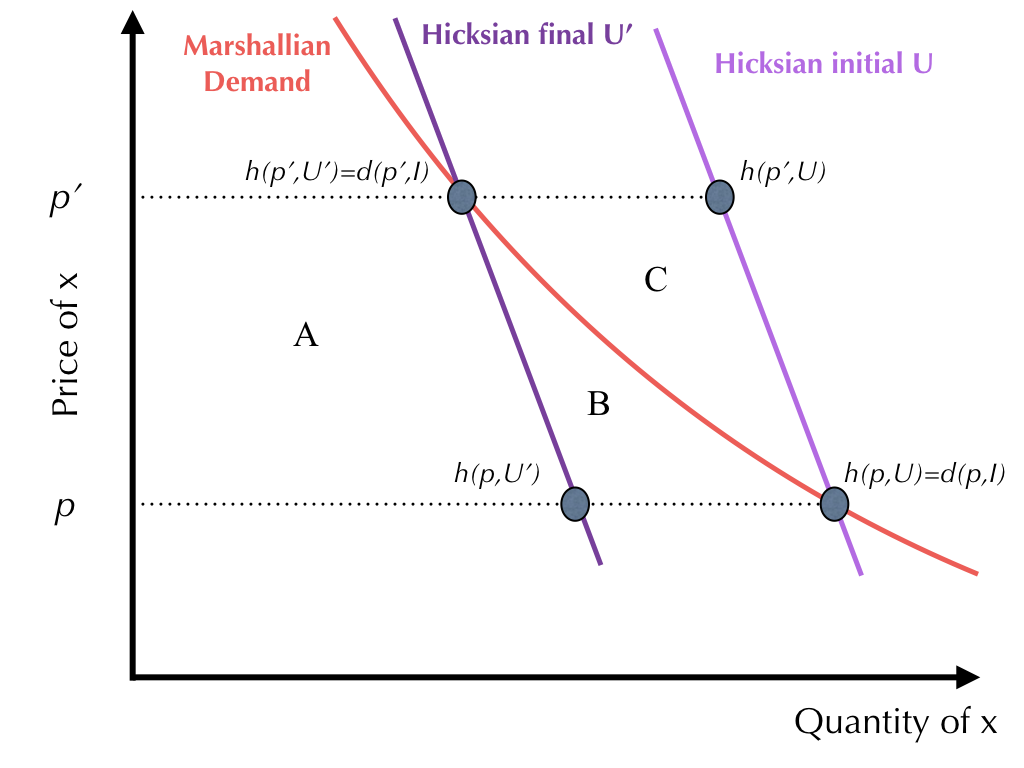
\includegraphics[scale=.3]{EVCV_normal.png}
\end{figure}
\FloatBarrier
Using the definitions above, $|EV|=A$,$|\Delta CS|=A+B$,$|CV|=A+B+C$
for the price increase, so we verify that $\mid CV\mid\geq\mid\Delta CS\mid\geq\mid EV\mid$
. We can see that the opposite chain of inequalities holds if we consider
a fall in price from $p'$ to $p$ in the same diagram, so that now
$|EV|=A+B+C$,$|\Delta CS|=A+B$,$|CV|=A$.

For an inferior good we get:
\FloatBarrier
\begin{figure}[!h]
%\centering{}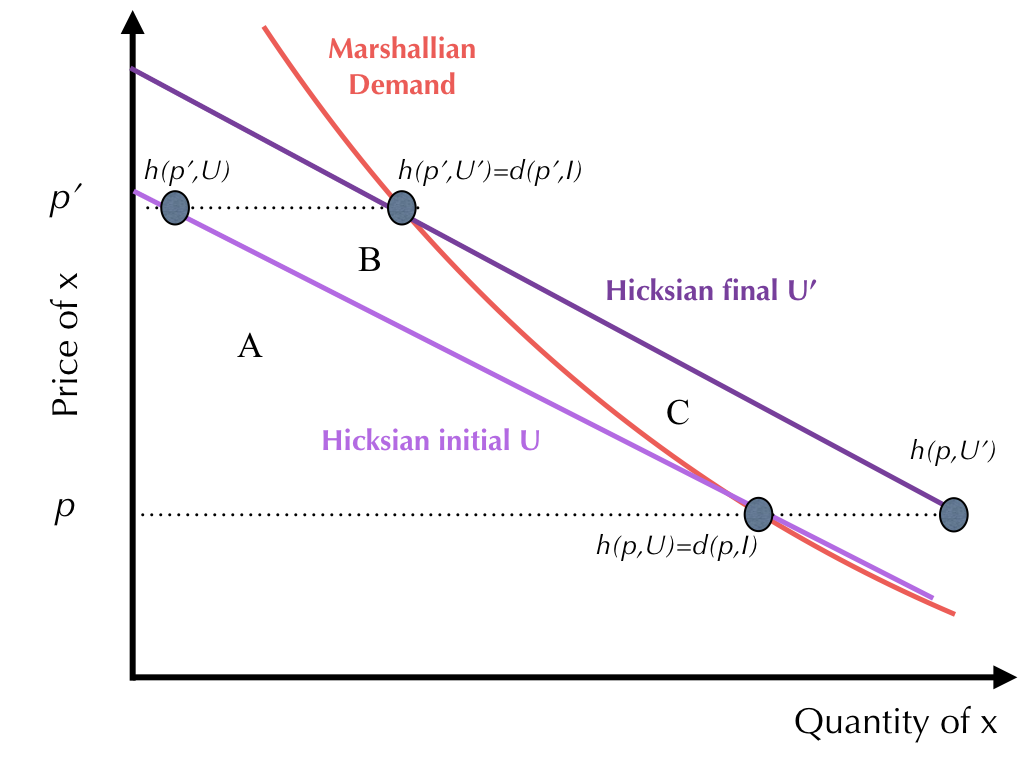
\includegraphics[scale=.3]{EVCV_inferior.png}
\end{figure}
\FloatBarrier
Using the definitions above, $|EV|=A+B+C$,$|\Delta CS|=A+B$,$|CV|=A$
for the price increase, verifying $\mid CV\mid\leq\mid\Delta CS\mid\leq\mid EV\mid$.

\subsection{Exercise}
\begin{itemize}
\item $U(x,y)=\sqrt{xy}$
\item One can solve the utility maximization and expenditure minimization
problem to get:
\begin{itemize}
\item $V(p_{x},p_{y},I)=\frac{I}{2\sqrt{p_{x}p_{y}}}$, $E(p_{x},p_{y},u)=2u\sqrt{p_{x}p_{y}}$
\item $d_{x}(p_{x},p_{y},I)=\frac{I}{2p_{x}}$ and $h_{x}(p_{x},p_{y},u)=u\sqrt{\frac{p_{y}}{p_{x}}}$
\end{itemize}
\item Suppose $I=8$, $p_{y}=4$, $p_{x}=$1.
\item Calculate CV, EV, and $\Delta$CS for the price increase of $x$ to
4 ($p_{x}^{'}=4$). 
\item We have that the Initial Marshallian demand for $x$ is: \textbf{$d_{x}(1,4,8)=\frac{8}{2}=4$}.
The initial Marshallian demand for $y$ is $d_{y}(1,4,8)=\frac{8}{8}=1$.
The initial utility is $U=V(1,4,8)=\frac{8}{2\sqrt{4}}=2$. Final
utility is: $U=V(4,4,8)=\frac{8}{2\sqrt{16}}=1$.
\item Note $h_{x}(p_{x},4,U')=h_{x}(p_{x},4,1)=1\sqrt{\frac{4}{p_{x}}}=2p_{x}^{-\frac{1}{2}}$,
and $h_{x}(p_{x},4,U)=h_{x}(p_{x},4,2)=2\sqrt{\frac{4}{p_{x}}}=4p_{x}^{-\frac{1}{2}}$
\item Thus, we can compute
\[
CV=\int_{1}^{4}h_{x}(p_{x},1,2)dp_{x}=4\int_{1}^{4}p_{x}^{-\frac{1}{2}}dp_{x}=8p_{x}^{\frac{1}{2}}\mid_{1}^{4}=16-8=8
\]
\item And:
\[
EV=\int_{1}^{4}h_{x}(p_{x},1,1)dp_{x}=2\int_{1}^{4}p_{x}^{-\frac{1}{2}}dp_{x}=4p\mid_{1}^{4}=8-4=4
\]
\item Finally:
\[
\Delta CS=\int_{1}^{4}d_{x}(p_{x},1,8)dp_{x}=4\int_{1}^{4}p_{x}^{-1}dp_{x}=4\log p_{x}\mid_{1}^{4}\approx5.54
\]
\end{itemize}

\end{document}
